\documentclass[10pt]{wlscirep}
\usepackage[utf8]{inputenc}
\usepackage[T1]{fontenc}
\usepackage{amsthm}
\usepackage{pythonhighlight}
\title{Review: "Build a Sporadic Group in Your Basement"}

\author[]{Parker Hyde}
\affil[]{Georgia State University, Mathematics and Statistics Department, Atlanta, 30302, U.S.A}
\affil[]{Email: phyde1@student.gsu.edu}

%\keywords{Keyword1, Keyword2, Keyword3}

\begin{abstract}
Example Abstract. Abstract must not include subheadings or citations. Example Abstract. Abstract must not include subheadings or citations. Example Abstract. Abstract must not include subheadings or citations. Example Abstract. Abstract must not include subheadings or citations. Example Abstract. Abstract must not include subheadings or citations. Example Abstract. Abstract must not include subheadings or citations. Example Abstract. Abstract must not include subheadings or citations.
\end{abstract}
\begin{document}

\flushbottom
\maketitle
% * <john.hammersley@gmail.com> 2015-02-09T12:07:31.197Z:
%
%  Click the title above to edit the author information and abstract
%
\thispagestyle{empty}

%\noindent Please note: Abbreviations should be introduced at the first mention in the main text � no abbreviations lists. Suggested structure of main text (not enforced) is provided below.

\section*{Introduction}


\paragraph{}

Any undergraduate student who has completed a course in abstract algebra will likely 
be familiar with the notion of a normal subgroup. A typical introductory textbook will introduce this 
concept early and 
%thoroughly 
emphasize its importance to many fundamental 
ideas such as homomorphisms, cosets, and Lagrange's Theorem. The 
%complementary 
relationship between normal groups and factor groups is often especially emphasized. 
Readers of I.N. Hernstein's Topics in Algebra, for example, will see a variety of examples in which
a normal subgroup N of a groups G, yields a factor group \( G / N \) comprised of cosets from 
the original group G.

\paragraph{}

The group of residue classes modulo 5, denoted by Z5, provides a particularly accessible 
example of this. This group can be obtained as a factor group, Z/5Z, from the group of integers 
Z with its associated normal subgroup 5Z. Reflecting on this example, an observant student 
might recognize that the group \( Z \) seems to permit a decomposition into a product of 
'simpler' groups 5Z and Z5 in the way that composite numbers can be decomposed into a product 
of smaller numbers. The student might further notice that Lagrange's Theorem forbids Z5 from 
having such a decomposition of its own due to its prime order. This might suggest that Z5,  
a cyclic group of order 5, is analogous to a prime number whose only factors are trivial. 
Thus the student may reasonably conclude that Z5 is some kind of special simple group in the 
sense that it is a finite group whose only proper normal subgroup is the trivial group. 
Indeed, such groups are called "finite simple groups" and they are of incredible importance 
in the modern mathematics landscape.

\paragraph{}

Tremendous effort and volumes of mathematical literature have been exhausted in trying to 
understand the so-called finite simple groups. A very large subset of this work, composed of 
over 10,000 pages written by more than 100 mathematicians, simply establishes a comprehensive
classification of the finite simple groups. Many mathematicians agree that this work is valid. 
The results show that almost every simple group falls into 1 or 18 infinite families[]. 
The first infinite family contains the group Z5 mentioned in out toy example above. 
In fact, it is comprised of all the cyclic groups of prime order. 
The second infinite family contains all alternating groups An, where n>=5. The remaining 16 
families are the groups of Lie type which are considerably more complex. Fascinatingly though, there 
exists 26 outlier simple groups known as the sporadic groups which fail to fit into 
any of these infinite families. 

\paragraph{}

The first 5 of these 26 exceptions to the rule were discovered by mathematician Emile Mathieu 
in 1873 and are appropriately named The Mathieu groups. Individually, the Mathieu groups are 
denoted \( M_{11},M_{12}, M_{22}, M_{23}, M_{24} \) where the subscripts signify that the 
Mathieu group \( M_n \) is a 
permutation group on n elements. The group \( M_{24} \) was originally instantiated by Mathieu as the 
the particular subgroup of \( S_{24} \) generated by the 3 arbitrary permutations:

\begin{align*}
    a &= (1, 2, 3, ..., 23) \\
    b &= (3, 17, 10, 7, 9)(5, 4, 13, 14, 19)(11, 12, 23, 8, 18)(21, 16, 15, 20, 22) \\
    c &= (1, 24)(2, 23)(3, 12)(4, 16)(5, 18)(6, 10)(7, 20) ...  (8, 14)(9, 21)(11, 17)(13, 22)(19, 15)
\end{align*}

This representation is generally opaque and leaves much to be desired for
a mathematician seeking a more natural construction. R.T Curtis, who presnted \( M_{24} \) as
group actions on an icosatetrahedron, stated that the construction was "clever" but "hardly natural."

\paragraph{}

Modern constructions of \( M_{24} \) 
are often defined as the automorphism group on one of two related finite structures. The first 
is the Steiner system S(5,8,24), a combinatorial block design. Two 
independent works by Witt and Carmichael showed that the automorphism group on this
structure is isomorphic to the permutation group generated by Mathieu. 
The second is the extended Golay error-correcting code and is of primary interest to this review
paper. The extended Golay code is distinct from the Steiner
System in its tangibility and practical applications. This feature makes the Golay code feel tractable
and presents a tempting target for reasearchers intersted in 
constructing \( M_{24} \). In the paper "Build a Sporadic Group in Your Basement", the 
authors attempt to leverage this by generating a representation for the automorphism on the 
extended Golay code that is "as simple" as possible." In doing so, they necessarily also generate a natural and enlightening 
construction for the Mathieu group \( M_{24} \).

\section*{Proofs and Results}

Building the Sporadic Group \( M_{24} \) will require some 
introductory results and definitions from coding theory. 
For this discussion, we
limit our scope to the algebraic properties of error-correcting codes and omit properties relevant to
engineering applications. These properties are interesting but they are not
relevant to the construction of \( M_{24} \). We begin with some notation and definitions.

%\subsubsection*{Coding Theory}
\medbreak
\noindent For simplicity, let \( F \) denote the field of binary numbers. Define addition and 
multiplication on this field by

\begin{figure}[ht]
    \centering
\begin{tabular}{|c|c|c|}
    \hline
    +&0&1\\
    \hline
    0&0&1\\
    \hline
    1&1&0\\
    \hline
\end{tabular}
\quad
\quad
\begin{tabular}{|c|c|c|}
    \hline
    x&0&1\\
    \hline
    0&0&0\\
    \hline
    1&0&0\\
    \hline
\end{tabular}
\caption{binary addition and multiplication tables for the field \( F \)}
\end{figure}


\theoremstyle{definition}
\newtheorem{definition}{Definition}
\begin{definition}[Binary Code]
    A \textit{Binary Code} with length \( n \) is a set of vectors  \( C = \{c_1, c_2, ..., c_m\} \)
    where each vector \( c_i \) \( i = 0, 1, ..., m \), is chosen from \( F^n \). 
    The vectors of this set are called \textit{Codewords}.
\end{definition} 


\noindent It follows from this definition that the set
\begin{align}
    S &= \{[0,0,0], [1,0,0], [0,1,0], [1,1,0]\}   
\end{align}

\noindent is a binary code of length \( 3 \). The vectors \( [0,0,0] \) and  \( [0,1,0] \) are
codewords of \( S \). 
\medbreak    
\noindent The code \( S \) also happens to be closed under vector addition and scalar multiplication.
In other words, \( S \) comprises a subspace of \( F^3 \). This property motivates our next definition.

\begin{definition}[Linear Binary Code]
    A \textit{Linear Binary Code} with dimension \( k \) is a binary code
    that completely exhausts a subspace of \( F^n \) with dimension \( k \).
\end{definition} 



\noindent Returning to our example, we see that the vectors \( [1,0,0] \) and  \( [0,1,0] \) form a basis
for the code \( S \). In particular, \( S \) contains all the vectors generated by that basis. Thus, we say \( S \) is a linear code with dimension \( 2 \). 

\bigbreak
\noindent It is customary to stack basis vectors for a code \( C \) as row vectors
in a \textit{generator matrix} \( M \). A valid generator matrix for \( S \) is 
\[
    M = \begin{bmatrix}
        1 & 0 & 0\\
        0 & 1 & 0
    \end{bmatrix}
\] 

\noindent Note that this generator matrix is not unique.

\bigbreak
\noindent Next, we address the \textit{minimum distance} for a linear code. 
The \textit{distance} between two codewords \( c_1 \) and \( c_2 \), denoted \( \text{dist}(c_1,c_2) \),
is the number of coordinates in which \( c_1 \) and \( c_2 \) differ. The \textit{weight} of 
a codeword \( c \), \( weight(c) \), is then defined to be dist(\( c, \textbf{0} \)), where \( \textbf{0} = [0, 0, ..., 0] \)
\medbreak
\newtheorem*{remark}{remark}
\begin{remark}
\noindent Usually, the minimum distance for a binary code \( C \) 
is the minimum value of the set \( \{\text{dist}(c_1, c_2) \mid c_1,c_2 \in C \} \). 
However for this reveiw, we are interested in linear codes. For linear codes, we always have that
\( \text{dist}(c_1,c_2) = \text{dist}(c_1 + c_2, 0) = \text{dist}(c_3, 0) \) from some \( c_3 \in C \). 
In this case, the minimum distance is just the smallest \( weight \) of any codeword \( c \in C\).
\end{remark}


\begin{definition}[Minimum Distance]
    The \textit{Minimum Distance} of a linear binary code is the 
    minimum value of \( \{ \text{weight}(c) \mid c \in C  \} \).

\end{definition} 

\noindent Up to this point, we have defined 3 important paramters of linear codes. These include
the \textit{length}, the \textit{dimension}, and the \textit{minimum distance}. We call a
linear code with length \( n \), dimension \( k \), and minimum distance \( d \) an \( (n,k,d) \)-code.

\subsection*{The Golay Code}
\bigbreak
The extended Golay Code will be instrumental in our construction of \( M_{24} \).
It is a linear binary \( (24,12,8) \)-code that was introduced by 
Marcel Golay in 1949. It is most easily assembled by the following greedy algorithm:
\medbreak
\noindent First, write down the numbers \(0, 1, 2, ..., 2^{24}-1 \) and consider
their representations as binary codewords of length 24. We will scan the list one by one and 
collect the codewords of the extended Golay code. Begin by adding \( 0 \) to the collection. 
This will be the first extended Golay codeword. Now scan the values  \( 1, 2, ..., 2^{n-1} \)
and add any value to the collection with distance at least \( 8 \) from any of the 
previously collected codewords. The resulting collection will be the extended Golay code.


\subsection*{Equivalent Codes and Automorphisms}
\medbreak
Recall that a homomorphism is a map \( f: A \to B \) that preverves an operation defined on the algebraic structures A and B. \linebreak
More formally, a map \( f: A \to B \) is a \textit{homomorphism} if there is a binary operation \( \mu \) defined on \( A \) and \( B \)
such that 
\[
    f(\mu_A(a_1,a_2)) = \mu_B(f(a_1), f(a_2))
\] 

\noindent for all \( a_1,a_2 \in A \).
\medbreak
\noindent Examples include linear maps which preserve linearity and group
homomorphism which preserve the group operation. We will be interested in 
homomorphisms on Linear Codes which preserve the distance operation.


\begin{definition}[Equivalent Linear Codes]
    Two Linear Binary Codes \( C \) and \( D \) of length \( n \) are \textit{equivalent}
    if a coordinate permutation on the codewords of \( C \) produces the codewords in \( D \).  
    More precisely, \( C \) and \( D \) are equivalent if there is a bijective map 
    \( \pi: C \to D \) where \( \pi(c) \) is a coordinate permutation on the codeword \( c \). 
\end{definition} 

\begin{remark}
    A coordinate permutation \( \pi: C \to D \) is a homomorphism which preserves the distance
    operation. In particular, 
\(
    \text{dist}(c_1,c_2) = \text{dist}(\pi(c_1), \pi(c_2))
\) 
\noindent for all \( c_1,c_2 \in C \).
\end{remark} 


\noindent An \textit{Automorphism} is a bijective homomorphism of the form 
\( f: A \to A \). Note that  \( f \) maps \( A \) back onto itself. 

\begin{definition}[Linear Code Automorphisms]
    An \textit{Automorphism} on a code \( C \) is a coordinate permutation
    \( \pi: C \to C \) which maps the codewords of \( C \) back \textit{onto} the codewords of \( C \).
\end{definition} 

\newtheorem{lemma}{Lemma}
\begin{lemma}
    A permutation that maps a basis for a code \( C \) to another basis is necessarily an automorphism on \( C  \).
    \textit{(proof omitted)}
\end{lemma} 

\begin{lemma}
    The set of automorphisms on a code \( C \) form a group under composition,
    denoted, Aut(\( C \)).
\end{lemma} 


\subsection*{The extended Golay code revisited}
\bigbreak

We will now explore some properties of the extended Golay code in light of \textit{equivalence} and 
\textit{automorphisms}.
Earlier we mentioned that the extended Golay code is an example of a \( (24,12,8) \)-code. We 
will see in the following theorem that any code with this property is equivalent to the 
extended Golay code.


\newtheorem{theorem}{Theorem}
\begin{theorem}[Pless]
    Let \( C \) be a linear binary \(  (24, 12, d)\)-code. Then the following
    statements are equivalent: \\
    \indent 1. The minimum weight of \( C \) is \( d \). \\
    \indent 2. \( C \) is equivalent to the extended Golay code.
\end{theorem}

\noindent We also state the following theorem which will serve as our
primary tool in constructing a natural representation for \( M_{24} \).

\begin{theorem}[Huffman, Pless]
    The full automorphism group of the extended
    binary Golay code, denoted Aut(\( G \)), is isomorphic to \( M_{24}\).
\end{theorem}

\noindent Theorem 2 has the natural consequence that any subgroup of Aut(\( G \)) will be
isomorphic to a subgroup of \( M_{24} \). This suggests a 
clever strategy for constructing \( M_{24} \). 
\medbreak
\noindent If we generate a group by composing two automorphisms of \( G \), 
then we are gauranteed the resulting subgroup will be isomorphic to a subgroup of \( M_{24} \).
Thus we might attempt to build \( M_{24} \) by choosing the 'right' pair of automorphisms on \( G \) in the hopes
that they might exhaust all elements of Aut(\( G \)). 
Such a pair would also generate \(M_{24} \).

\bigbreak

\subsection*{Building the Sporadic Group}
\medbreak
\noindent We now have the necessary vocabulary to disscuss a construction of \( M_{24} \). In fact, we will
simply build the group outright. 
\medbreak
\noindent After developing and expanding on the coding theory which
we have just presented, the authors of "Build a Sporadic Group in Your Basement"
eventually arrive at the following construction for \( M_{24} \). 
The result is a subgroup of the symmetric group \( S_{24} \) generated by two 
permutation:
\begin{align*}
    \tau &= (1, 2, 3, 4, 5, 15, 19, 11, 10, 9, 12, 7, 13, 14, 23, 24, 17, 18, 22, 6, 21, 8, 20)(16)  \\ 
    \rho &= (1, 2, 3)(4, 5, 6) ... (22, 23, 24) \\
\end{align*}

\noindent The software package \textbf{GAP} was used to verify that the group generated by
\( \tau \) and \( \rho \) is simple with 244,823,040 elements. This fact along with 
the following lemma stated in the paper is illuminating.

\begin{lemma}
    The only simple group of order 244, 823, 040 is the Mathieu group \( M_{24} \).
\end{lemma}

\noindent The group constructed by \( \tau \) and \( \rho \) is the Mathieu group \( M_{24} \).
We will now attempt to uncover how the authors arrived at this construction. In doing so, we
will also provide an alternate proof that this is \( M_{24} \) through the avenue of 
Theorem 2. In particular, we show that \( \tau \) and \( \rho \) are both automorphisms on 
the extended Golay code.
\bigbreak

\noindent To this end we introduce two new models of the extended Golay code.

\subsection*{Quadratic Residue Model (R)}
\medbreak
\noindent The Quadratic Residue model is almost exactly the model originally proposed by
Marcel Golay. The generator matrix for the code is produced by the set \( \{ 1, 2, 3, 4, 6, 8, 9, 12, 13, 16, 18 \} \),
the set of numbers  \( q \) which allow integers solutions to
the equation \( x^2 \equiv q \) (mod \( 23 \)). 
The first codeword in the generator matrix is the vector with ones in these positions,
an additional one in position \( 24 \), and the remaining positions zero. The next
11 rows are generated by applying the permutation
\[
    \sigma = (1, 2, 3, 4, 5, 15, 19, 11, 10, 9, 12, 7, 13, 14, 23, 24, 17, 18, 22, 6, 21, 8, 20)(16)\\ 
\] 


\noindent to the previously generated row. This yields the generator matrix:
\setcounter{MaxMatrixCols}{25}
\setlength\arraycolsep{0.5pt}

\[
    Q = \begin{bmatrix}
        1&1&1&1&0&1&0&1&1&0&0&1&1&0&0&1&0&1&0&0&0&0&0& & 1 \\
        0&1&1&1&1&0&1&0&1&1&0&0&1&1&0&0&1&0&1&0&0&0&0& & 1 \\
        0&0&1&1&1&1&0&1&0&1&1&0&0&1&1&0&0&1&0&1&0&0&0& & 1 \\
        0&0&0&1&1&1&1&0&1&0&1&1&0&0&1&1&0&0&1&0&1&0&0& & 1 \\
        0&0&0&0&1&1&1&1&0&1&0&1&1&0&0&1&1&0&0&1&0&1&0& & 1 \\
        0&0&0&0&0&1&1&1&1&0&1&0&1&1&0&0&1&1&0&0&1&0&1& & 1 \\
        1&0&0&0&0&0&1&1&1&1&0&1&0&1&1&0&0&1&1&0&0&1&0& & 1 \\
        0&1&0&0&0&0&0&1&1&1&1&0&1&0&1&1&0&0&1&1&0&0&1& & 1 \\
        1&0&1&0&0&0&0&0&1&1&1&1&0&1&0&1&1&0&0&1&1&0&0& & 1 \\
        0&1&0&1&0&0&0&0&0&1&1&1&1&0&1&0&1&1&0&0&1&1&0& & 1 \\
        0&0&1&0&1&0&0&0&0&0&1&1&1&1&0&1&0&1&1&0&0&1&1& & 1 \\
        1&0&0&1&0&1&0&0&0&0&0&1&1&1&1&0&1&0&1&1&0&0&1& & 1\\ 
    \end{bmatrix}
\] 

A moderate amount of python code shows that the permutation \( \sigma \) maps the final
row of \( Q \) to the vector sum of columns 1,2,3,4,5,8, and 11. This is the only
combination of basis codewords in \( Q \) which achieves this. Thus \( \sigma \) maps
the basis codewords of \( Q \) to a new linearly independent basis. By Lemma 1, \( \sigma \) is automorphism
on the extended Golay code.

\subsection*{Block-Substitution Model (B)}
\medbreak
\noindent We now turn our attention to the Block-Substitution model of the Golay code.
This model was introduced by the authors of "Build a Sporadic Group in Your Basement."
We proceed by substituting the \( 3 x 3  \) matrix blocks

\setlength\arraycolsep{4pt}
\[
    I = \begin{bmatrix}
        1 & 0 & 0\\
        0 & 1 & 0\\
        0 & 0 & 1
    \end{bmatrix},
    \quad
    \overline{I} = \begin{bmatrix}
        0 & 1 & 1\\
        1 & 0 & 1\\
        1 & 1 & 0
    \end{bmatrix}
    \quad
    J = \begin{bmatrix}
        1 & 1 & 1\\
        1 & 1 & 1\\
        1 & 1 & 1
    \end{bmatrix}
    \quad
    \text{into the matrix}
    \quad
    G = \begin{bmatrix}
        I & 0 & 0 & 0 & \overline{I} & I & I & J\\
        0 & I & 0 & 0 & J & \overline{I} & I & I\\
        0 & 0 & I & 0 & I & J & \overline{I} & I\\
        0 & 0 & 0 & I & I & I & J & \overline{I}
    \end{bmatrix}
\] 

\noindent to obtain

\setlength\arraycolsep{0.5pt}
\[
    G = \begin{bmatrix}
        1&0&0&0&0&0&0&0&0&0&0&0&0&1&1&1&0&0&1&0&0&1&1&1\\
        0&1&0&0&0&0&0&0&0&0&0&0&1&0&1&0&1&0&0&1&0&1&1&1\\
        0&0&1&0&0&0&0&0&0&0&0&0&1&1&0&0&0&1&0&0&1&1&1&1\\
        0&0&0&1&0&0&0&0&0&0&0&0&1&1&1&0&1&1&1&0&0&1&0&0\\
        0&0&0&0&1&0&0&0&0&0&0&0&1&1&1&1&0&1&0&1&0&0&1&0\\
        0&0&0&0&0&1&0&0&0&0&0&0&1&1&1&1&1&0&0&0&1&0&0&1\\
        0&0&0&0&0&0&1&0&0&0&0&0&1&0&0&1&1&1&0&1&1&1&0&0\\
        0&0&0&0&0&0&0&1&0&0&0&0&0&1&0&1&1&1&1&0&1&0&1&0\\
        0&0&0&0&0&0&0&0&1&0&0&0&0&0&1&1&1&1&1&1&0&0&0&1\\
        0&0&0&0&0&0&0&0&0&1&0&0&1&0&0&1&0&0&1&1&1&0&1&1\\
        0&0&0&0&0&0&0&0&0&0&1&0&0&1&0&0&1&0&1&1&1&1&0&1\\
        0&0&0&0&0&0&0&0&0&0&0&1&0&0&1&0&0&1&1&1&1&1&1&0\\
    \end{bmatrix}
\] 

\bigbreak
\noindent
Again, we will seek an automorphism that preserves the basis codewords of our generator matrix
\( G \). The cyclic structure of the blocks \( I \), \(\overline{I} \), and \( J \) suggests the 
permutation
\[
    \rho = (1, 2, 3)(4, 5, 6) ... (22, 23, 24) \\
\] 
Indeed, this permutation completely preserves the row vectors of \( G \). Moreover, it is one
of the two permutation we saw early which the authors use to build \( M_{24} \). 

\subsection*{Equivalence of Quadratic Residue and Block-Substitution models}
\bigbreak
\noindent
We now have two automorphisms, \( \sigma \) and \( \rho \), which operate on distinct Golay
code models \( R \) and \( B \).
\smallbreak
\noindent
Both of these permutations fell naturally, if not trivially, out of their respective Golay code models. 
The prevailing sentiment in BSGYB is that
the models \( R \) and \( B \) might be "different" enough that their corresponding automorphisms
capture the information needed to
generate the Golay code automorphism group.
We might be tempted
to compose these permutations directly to this end. However this approach
would be meaningless. \( \sigma \) and \( \rho \) operate on 
distict codes so they do not preserve any useful structure.

\medbreak
\noindent 
Instead we will seek an equivalence map between \( R \) and \( B \). The resulting map can 
then be used to express \( \sigma \) in terms of the code  \( B \).
Recall from Theorem 1 that any \( (24,12,8) \)-code is equivalent to the extended
Golay code. It follows from this that an equivalence map must exist between  \( R \) and \( B \).
We will still need to find this map if we wish to express \( \sigma \) in the language 
of the code \( B \).


% we will skip a detailed derivation

% guesswork. we will avoid the scenic route

\begin{python}
\end{python}



%\item First item
%\item Second item
%\end{itemize}


\section*{Discussion}

The Discussion should be succinct and must not contain subheadings.

\section*{Methods}

Topical subheadings are allowed. Authors must ensure that their Methods section includes adequate experimental and characterization data necessary for others in the field to reproduce their work.

\bibliography{sample}

\noindent LaTeX formats citations and references automatically using the bibliography records in your .bib file, which you can edit via the project menu. Use the cite command for an inline citation, e.g.  \cite{Hao:gidmaps:2014}.

For data citations of datasets uploaded to e.g. \emph{figshare}, please use the \verb|howpublished| option in the bib entry to specify the platform and the link, as in the \verb|Hao:gidmaps:2014| example in the sample bibliography file.

\section*{Acknowledgements (not compulsory)}

Acknowledgements should be brief, and should not include thanks to anonymous referees and editors, or effusive comments. Grant or contribution numbers may be acknowledged.

\section*{Author contributions statement}

Must include all authors, identified by initials, for example:
A.A. conceived the experiment(s),  A.A. and B.A. conducted the experiment(s), C.A. and D.A. analysed the results.  All authors reviewed the manuscript. 

\section*{Additional information}

To include, in this order: \textbf{Accession codes} (where applicable); \textbf{Competing interests} (mandatory statement). 

The corresponding author is responsible for submitting a \href{http://www.nature.com/srep/policies/index.html#competing}{competing interests statement} on behalf of all authors of the paper. This statement must be included in the submitted article file.

\begin{figure}[ht]
\centering
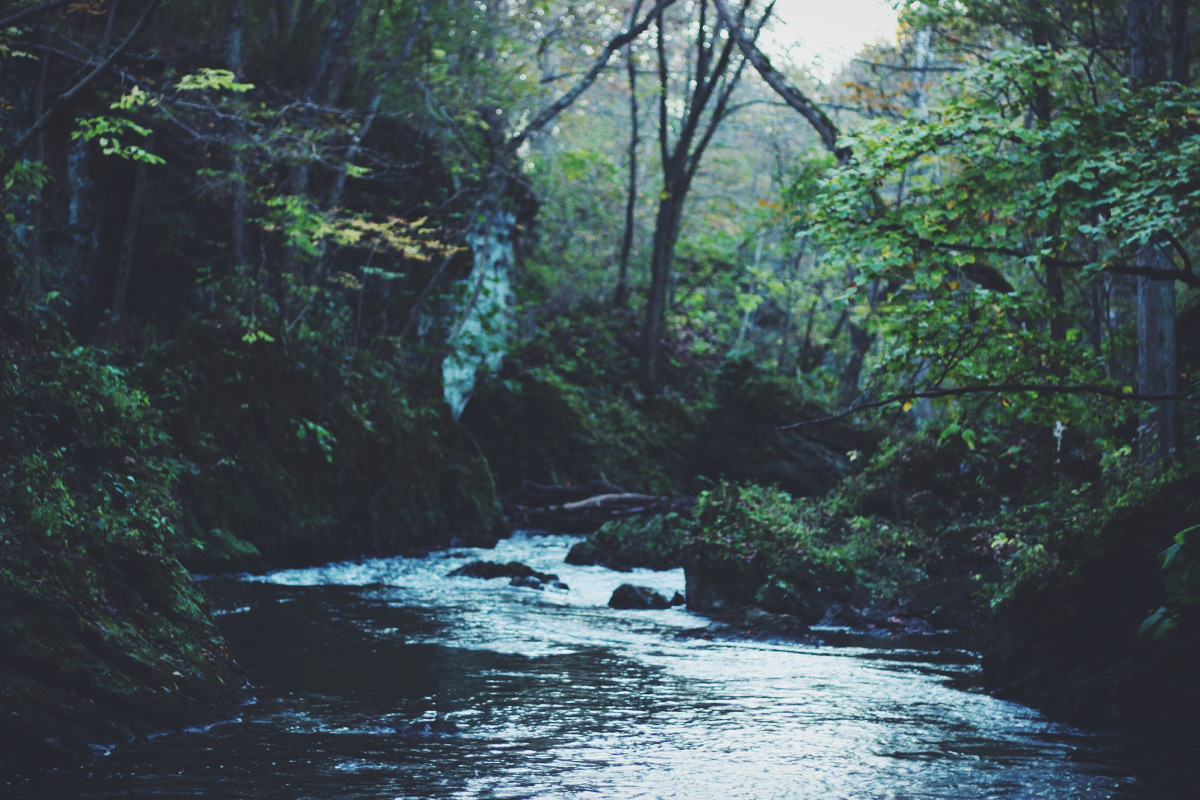
\includegraphics[width=\linewidth]{stream}
\caption{Legend (350 words max). Example legend text.}
\label{fig:stream}
\end{figure}

\begin{table}[ht]
\centering
\begin{tabular}{|l|l|l|}
\hline
Condition & n & p \\
\hline
A & 5 & 0.1 \\
\hline
B & 10 & 0.01 \\
\hline
\end{tabular}
\caption{\label{tab:example}Legend (350 words max). Example legend text.}
\end{table}

Figures and tables can be referenced in LaTeX using the ref command, e.g. Figure \ref{fig:stream} and Table \ref{tab:example}.

\end{document}
